\chapter{Theoretical Basis for CFAST}

Adequately detailed documentation of the theoretical basis of the model allows the model user to
understand the underlying theory behind the model implementation and thus be able to assess the
appropriateness of the model to specific problems. This chapter presents a derivation of the
predictive equations for zone fire models and explains in detail the ones used in CFAST.

The modeling equations used in CFAST take the mathematical form of an initial value problem
for a system of ordinary differential equations. These equations are derived using the
conservation of mass, the conservation of energy (equivalently the first law of thermodynamics),
the ideal gas law. These equations predict as functions of time quantities such as pressure, layer
height and temperatures given the accumulation of mass and enthalpy in the two layers. The
assumption of a zone model is that properties such as temperature can be approximated
throughout a control volume by an average value.

Many formulations based upon these assumptions can be derived. One formulation can be
converted into another using the definitions of density, internal energy and the ideal gas law.
Though equivalent analytically, these formulations differ in their numerical properties. Each
formulation can be expressed in terms of mass and enthalpy flow. These rates represent the
exchange of mass and enthalpy between zones due to physical phenomena such as plumes,
natural and forced ventilation, convective and radiative heat transfer, and so on. For example, a
vent exchanges mass and enthalpy between zones in connected rooms, a fire plume typically
adds heat to the upper layer and transfers entrained mass and enthalpy from the lower to the
upper layer, and convection transfers enthalpy from the gas layers to the surrounding walls.

As discussed in references \cite{Forney:1992} and \cite{Rehm:1992}, the zone fire modeling ordinary differential equations (ODEs) are stiff. The term stiff means that large variations in time scales are present in the ODE
solution. In our problem, pressures adjust to changing conditions more quickly than other
to solve zone fire modeling ODEs because of this stiffness. Runge-Kutta methods or predictorcorrector
methods such as Adams-Bashforth require prohibitively small time steps in order to
track the short-time scale phenomena (pressure in our case). Methods that calculate the Jacobian
(or at least approximate it) have a much larger stability region for stiff problems and are thus
more successful at their solution.


\section{Derivation of Equations for a Two-Layer Model}

A compartment is divided into two control volumes, a relatively hot upper layer and a relatively cool lower layer, as illustrated in figure \ref{fig:Control_Volumes}.  The gas in each layer has attributes of mass, internal energy, density, temperature, and volume denoted respectively by $m_i$, $E_i$, $\rho_i$, $T_i$, and $V_i$ where $i$=$L$ for the lower layer and $i$=$U$ for the upper layer.  The compartment as a whole has the attribute of pressure $P$.  These 11 variables are related by means of the following seven constraints (counting density, internal energy and the ideal gas law twice, once for each layer).

\be \rho _i  = \frac{{m_i }}{{V_i }} {\hspace{1.0in} \textnormal{Density}} \label{eq:density} \ee

\be  E_i = c_v m_i T_i {\hspace{1.0in} \textnormal{Internal Energy}} \label{eq:internal_energy} \ee

\be P = R\rho _i T_i {\hspace{1.0in} \textnormal{Ideal Gas Law}} \ee

\be V = V_L + V_U {\hspace{1.0in} \textnormal{Total Volume}} \label{eq:volume} \ee

\begin{figure}[h]
\begin{center}
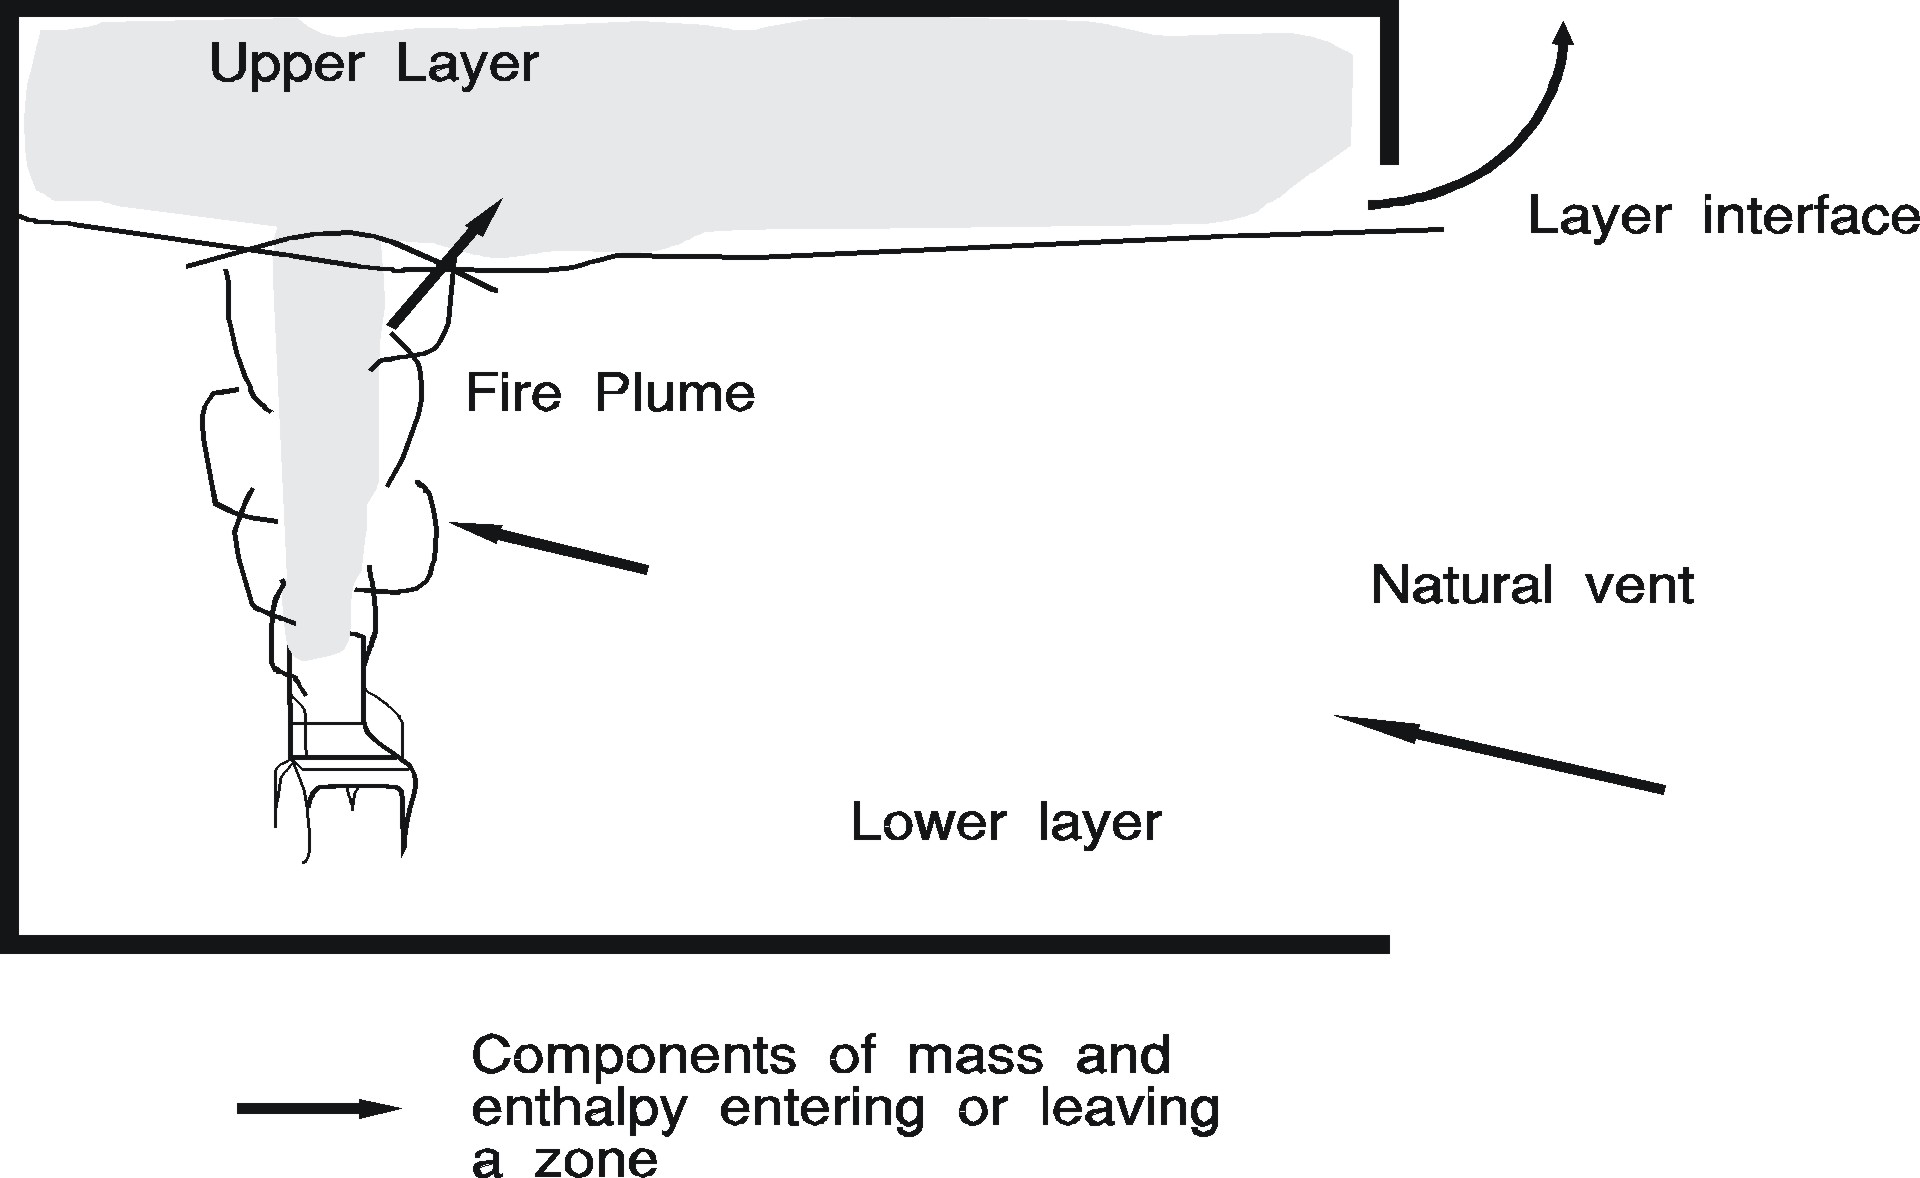
\includegraphics[width=4.0in]{FIGURES/Theory/Control_Volumes}\\
\end{center}
\caption{Schematic of control volumes in a two-layer zone model.}
 \label{fig:Control_Volumes}
\end{figure}

The specific heat at constant volume and at constant pressure $c_v$ and cp, the universal gas constant, R, and the ratio of specific heats, $\gamma$, are related by $\gamma = c_p / c_v$ and $R = c_p- c_v$.  For ambient air, $c_p \approx 1$ kJ/kg K and $\gamma = 1.4$.  Four additional equations obtained from conservation of mass and energy for each layer are required to complete the equation set.  The differential equations for mass in each layer are 

\be \frac{{dm_L }}{{dt}} = \dot m_L \ee

\be \frac{{dm_U }}{{dt}} = \dot m_U \ee

The first law of thermodynamics states that the rate of increase of internal energy plus the rate at
which the layer does work by expansion is equal to the rate at which enthalpy is added to the gas.
In differential form this is

\be \begin{array}{ccccc}
   {{\textnormal{internal energy}}} & {} & {{\textnormal{work}}} & {} & {{\textnormal{enthalpy}}}  \\
   {\overbrace {}^{}} & {} & {\overbrace {}^{}} & {} & {\overbrace {}^{}}  \\
   {\displaystyle {\dbydt{E_i}}} &  +  & {P \displaystyle {\dbydt{V_i}}} &  =  & {\dot h_i }  \\
\end{array} \label{eq:first_law} \ee

where $c_p$ is taken as constant in the enthalpy term,

\be \dot h = c_p \dot m_U T_U + \dot E_U + c_p \dot m_LT_L + \dot E_L \ee

A differential equation for pressure can be derived by adding the upper and lower layer versions
of eq (\ref{eq:first_law}), noting that $\dbydt{V_U} = -\dbydt{V_L}$, and that

\be \dbydt{E_i} = \dbydt{ \brackets{c_v \dot m_i T_i}} = \frac{{c_v}}{{R}} \dbydt{ \brackets{PV_i}} \label{eq:differential_internal_energy}  \ee

to obtain

\be \dbydt{P} = \frac{{\gamma -1}}{{V}} \brackets{\dot h_L + \dot h_U}  \ee

Differential equations for the layer volumes can be obtained by substituting equation \ref{eq:differential_internal_energy} into \ref{eq:first_law} to obtain

\be \dbydt{V_i} = \frac{1}{P \gamma} \brackets{\brackets{\gamma -1} \dot h_i - V_i \dbydt{P}} \label{eq:layer_volume} \ee

Equation \ref{eq:internal_energy} can be rewritten using eq \ref{eq:layer_volume} to eliminate $dV/dt$ to yield

\be \dbydt{E_i} = \frac{1}{\gamma} \brackets{\dot h_i + V \dbydt{P}} \ee

A differential equation for density can be derived by applying the quotient rule to $\frac{d \rho_i}{dt} = \frac{d}{dt} \brackets{\frac{m_i}{V_i}}$ and using eq \ref{eq:layer_volume} to eliminate $\frac{dV_i}{dt}$ to obtain

\be \dbydt{\rho_i} = \frac{-1}{c_p T_i V_i} \brackets{\brackets{\dot h_i - c_p \dot m_i T_i} - \frac{V_i}{\gamma - 1}\dbydt{P}} \label{eq:layer_density}\ee

Temperature differential equations can be obtained from the equation of state by applying the quotient rule to $\dbydt{T_i} = \dbydt{} \brackets{\frac{P}{R \rho_i}}$ and using eq \ref{eq:layer_density} to eliminate $\dbydt{\rho_i}$ to obtain

\be \dbydt{T_i} = \frac{1}{c_p rho_i V_i} \brackets{\brackets{\dot h_i - c_p \dot m_i T_i}+ V_i \dbydt{P}} \ee

These equations for each of the 11 variables are summarized in table \ref{tab:zone_model_equations}. The time evolution of
these solution variables can be computed by solving the corresponding differential equations
together with appropriate initial conditions. The remaining seven variables can be determined
from the four solution variables using eqs (\ref{eq:density}) to (\ref{eq:volume}).

\begin{table}
\begin{center}
\caption{Conservative zone model equations}
\label{tab:zone_model_equations}
\vspace{0.1in}
\begin{tabular}{|c|c|}
\hline
Equation Type & Differential Equation \\ \hline
i'th layer mass & $\displaystyle {\dbydt{m_i} = \dot m_i}$ \\ \hline
pressure & $\displaystyle {\dbydt{P} = \frac{{\gamma -1}}{{V}} \brackets{\dot h_L + \dot h_U}}$ \\ \hline
i'th layer energy & $\displaystyle {\dbydt{E_i} = \frac{1}{\gamma} \brackets{\dot h_i + V \dbydt{P}}}$ \\ \hline
i'th layer volume & $\displaystyle {\dbydt{V_i} = \frac{1}{P \gamma} \brackets{\brackets{\gamma -1} \dot h_i - V_i \dbydt{P}} }$ \\ \hline
i'th layer density & $\displaystyle {\dbydt{\rho_i} = \frac{-1}{c_p T_i V_i} \brackets{\brackets{\dot h_i - c_p \dot m_i T_i} - \frac{V_i}{\gamma - 1}\dbydt{P}}}$ \\ \hline
i'th layer temperature & $\displaystyle {\dbydt{T_i} = \frac{1}{c_p rho_i V_i} \brackets{\brackets{\dot h_i - c_p \dot m_i T_i}+ V_i \dbydt{P}}}$ \\ \hline
\end{tabular}  
\end{center}
\end{table}

There are, however, many possible differential equation formulations. Indeed, there are 330
different ways to select four variables from eleven. Many of these systems are incomplete due to
the relationships that exist between the variables given in eqs (\ref{eq:density}) to (\ref{eq:volume}). For example the
variables, $\rho_U$, $V_U$, $m_U$, and $P$ form a dependent set since $\rho_U = m_U / V_U$.

The number of differential equation formulations can be considerably reduced by not mixing
variable types between layers; that is, if upper layer mass is chosen as a solution variable, then
lower layer mass must also be chosen. For example, for two of the solution variables choose $m_L$
and $m_U$, or $\rho_L$ and $\rho_U$, or $T_L$ and $T_U$. For the other two solution variables pick $E_L$ and $E_U$ or $P$ and $V_L$ or $P$ and $V_U$. This reduces the number of distinct formulations to nine. Since the numerical properties of the upper layer volume equation are the same as a lower layer one, the number of
distinct formulations can be reduced to six.

\section{Equation Set Used in CFAST}

The current version of CFAST is set up to use the equation set for layer temperature, layer
volume, and pressure as shown below.

\be \dbydt{P} = \frac{{\gamma -1}}{{V}} \brackets{\dot h_L + \dot h_U}  \ee

\be \dbydt{V_U} = \frac{1}{P \gamma} \brackets{\brackets{\gamma -1} \dot h_i - V_U \dbydt{P}} \ee

\be \dbydt{T_U} = \frac{1}{c_p rho_i V_U} \brackets{\brackets{\dot h_U - c_p \dot m_U T_U}+ V_U \dbydt{P}} \ee

\be \dbydt{T_L} = \frac{1}{c_p rho_i V_L} \brackets{\brackets{\dot h_L - c_p \dot m_L T_L}+ V_L \dbydt{P}} \ee

In these equations, the pressure is actually modeled with the pressure difference relative to an
ambient reference pressure to minimize numerical instability.

\section{Limitations of the Zone Model Assumptions}

The basic assumption of all zone fire models is that each compartment can be divided into a
small number of control volumes, each of which is uniform in temperature and composition. In
CFAST all compartments have two zones except for the fire room which has an additional zone
for the plume. Since a real upper/lower interface is not as sharp as this, one has a spatial error of
about 10~\% in determining the height of the layer \cite{Steckler:1982, Quintiere:1984}.

The zone model concept best applies for an enclosure in which the width and length are not too
different. If the horizontal dimensions of the room differ too much (i.e., the room looks like a
corridor), the flow pattern in the room may become asymmetrical. If the enclosure is too
shallow, the temperature may have significant radial differences. The width of the plume may at
some height become equal to the width of the room and the model assumptions may fail in a tall
and narrow enclosure. Therefore, the user should recognize approximate limits on the ratio of the
length ($L$), width ($W$), and height ($H$) of the compartment.

If the aspect ratio (length/width) is over about 10, the corridor flow algorithm should be used.
This provides the appropriate filling time. Similarly, for tall shafts (elevators and stairways), a
single zone approximation is more appropriate. It was found experimentally \cite{Klote:1990} that the mixing
between a plume and lower layer due to the interaction with the walls of the shaft, caused
complete mixing. The is the flip side of the corridor problem and occurs at a ratio of the height
to characteristic floor length of about 10. The following quantitative limits are recommended:

\begin{table}[h]
\begin{center}
\caption{Recommended compartment dimension limits}
\label{tab:compartment_limits}
\vspace{0.1in}
\begin{tabular}{|c|c|c|c|}
\hline
Group & Acceptable & Special consideration & Corridor flow \\ 
 & & required & algorithm \\ \hline
$(L/W)_{max}$ & $L/W < 3$ & $3 < L/W < 5$ & $L/W > 5$ \\ \hline
$(L/H)_{max}$ &  $L/H < 3$ & $3 < L/H < 6$ & $L/H > 6$ \\ \hline
 $(W/H)_{max}$ & $W/H > 0.4$ & $0.2 < L/W < 0.4$ & $L/W < 0.2$ \\ \hline
\end{tabular}  
\end{center}
\end{table}

\section{Source Terms for the Model}

This section discusses each of the sub-models in CFAST. In general, the sections are similar to
the way the model itself is structured. The sub-sections which follow discuss the way the actual
phenomena are implemented numerically. For each of the phenomena discussed below, the
physical basis for the model is discussed first, followed by a brief presentation of the
implementation within CFAST. For all of the phenomena, there are basically two parts to the
implementation: the physical interface routine (which is the interface between the CFAST
model and the algorithm) and the actual physical routine(s) which implement the physics. This
implementation allows the physics to remain independent of the structure of CFAST and allows
easier insertion of new phenomena.

\subsection{The Fire}

A fire in CFAST is implemented as a source of fuel mass which is released at a prescribed rate
(the pyrolysis rate). Energy is released by the fuel and combustion products are created as it
burns.

The model can simulate multiple fires in one or more compartments of the building. These fires
are treated as totally separate entities, with no interaction of the plumes. These fires are generally
referred to as ``objects'' and can be ignited at a prescribed time, temperature or heat flux.

CFAST does not include a pyrolysis model to predict fire growth. Rather, pyrolysis rates for
each fire are prescribed by the user. While this approach does not directly account for increased
pyrolysis due to radiative feedback from the flame or compartment, in theory these effects could
be prescribed by the user. In an actual fire, this is an important consideration, and the
specification used should consider the experimental conditions as closely as possible.

\subsubsection{Constrained Fire}

A fire releases energy based on the pyrolysis of fuel, but may be constrained by the oxygen
available for combustion depending on the compartment conditions. Complete burning will take
place only where there is sufficient oxygen. When insufficient oxygen is entrained into the fire
plume, unburned fuel will be transported from zone to zone until there is sufficient oxygen and a
high enough temperature to support combustion. In general, CFAST uses a simple definition of
a combustion reaction that includes major products of combustion for hydrocarbon fuels:

\be  \mathrm{C_xH_yO_zN_aCl_b} +  \nu_\OTWO \, \mathrm{O_2}  \rightarrow  \nu_\COTWO \, \mathrm{CO_2} + \nu_\HTWOO \, \mathrm{H_2O} + \nu_\CO \, \mathrm{CO} +
     \nu_\So \, \mathrm{Soot}  + \nu_\NTWO \, \mathrm{N_2} + \nu_\HCl \mathrm{HCl} + \nu_\HCN \mathrm{HCN} \label{stoich} \ee     
where the stoichiometric coefficients $\nu\OTWO$, $\nu_\COTWO$, etc. represent appropriate molar ratios for a stoichiometric balance of the equation.  For example, for soot, it is related to the
{\em soot yield}, $y_\So$, via the relation:
\be
   \nu_\So = \frac{W_\F}{W_\So} \; y_\So \label{soot_yield}
\ee

For complete combustion of the simplest hydrocarbon fuel, methane reacts with 
oxygen to form carbon dioxide and water. The only input required is the pyrolysis rate and the 
heat of combustion. For fuels that contain oxygen, nitrogen, or chlorine, the reaction becomes 
more complex. In this case, production yields for the species are prescribed by the user. 
Stoichiometry is used to insure conservation of mass and elements in the reaction. The species 
which are calculated are oxygen, carbon dioxide, carbon monoxide, water, and soot. Gaseous nitrogen is included, but only acts as a diluent. Production of hydrogen cyanide and hydrogen chloride are tracked solely based on user prescribed yields. The heat release rate for a constrained fire may be reduced below its prescribed value based upon the oxygen available for combustion.  When there is not enough oxygen to support complete combustion, some of the fuel will be transported to the gas layers and through vents as unburned hydrocarbons.

As fuel and oxygen are consumed, heat is released and various products of combustion are formed. The heat is released as radiation and convected enthalpy:

\begin{eqnarray} Q_{f,R} &=& \chi_R Q_f \\
Q_{f,R} &=& \brackets{1-\chi_R} Q_f
\end{eqnarray}
where, $\chi_R$ is the fraction  of the fire�s heat release rate given off as radiation.  The convective 
enthalpy, $Q_{f,C}$ then becomes the driving term in the plume flow.  For a constrained fire there is 
radiation to both the upper and lower layers, whereas the convective part contributes only to the 
upper layer.

\subsubsection{Limiting Combustion by Available Oxygen}

For any individual fire, the heat release rate is limited by available oxygen in the layer where the fire is located. This limit is applied in three 
places, which are shown schematically in figure 3. The first is burning in the portion of the 
plume which (at least initially) is typically in the lower layer of the room of fire origin (region \# 1).  The second is the portion of the plume in the upper layer, also in the room of origin (region \# 2).  The third is in the 
vent flow which entrains air from a lower layer into an upper layer in an adjacent compartment 
(region \# 3). The unburned hydrocarbons are tracked in this model.  Further combustion of CO to 
$\mathrm{CO_2}$ is not included in the model.

\begin{figure}[h]
\begin{center}
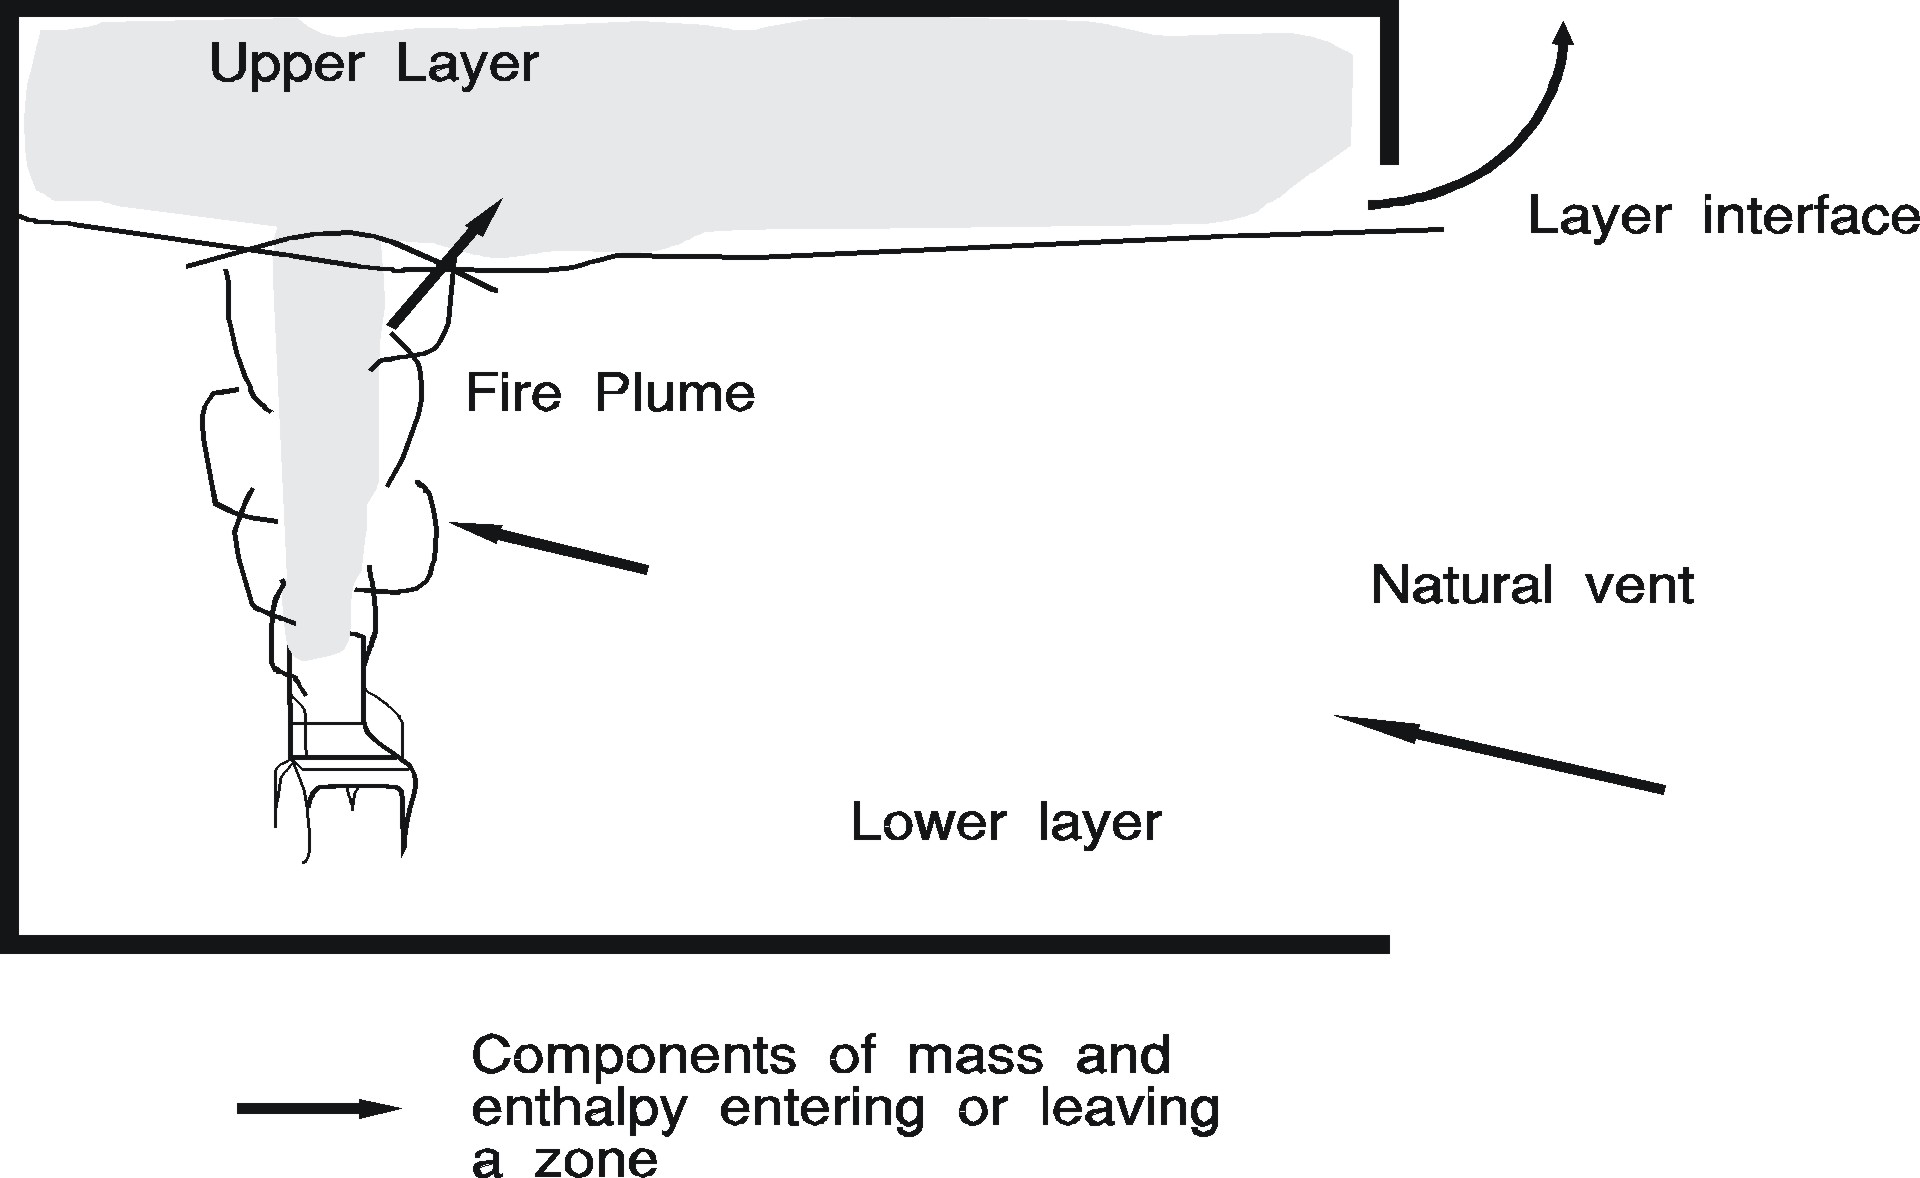
\includegraphics[width=4.0in]{FIGURES/Theory/Control_Volumes}\\
\end{center}
\caption{Entrainment and burning in a two-layer, multi-compartment model.}
 \label{fig:Burning_Regions}
\end{figure}

Initially, $\dot{m_f}$ is just the pyrolysis rate of the source fire in kg/s (region \# 1). For subsequent regions, the burning rate $\dot{m_f}$ is the unburned fuel from a previous region, $\dot{m_{tuhc}} = \dot{m_f} - \dot{m_b}$ where the subscript $tuhc$ is total unburned hydrocarbons, $f$ is the fire source, and $b$ is the amount burned.

The first step is to limit the actual burning which takes place in the combustion zone.  In each 
combustion zone, there is a quantity of fuel available.  At the source this results from the 
pyrolysis of the material, $\dot{m}_f$ .  In other situations such as a plume or door jet, it is the net 
unburned fuel available, $\dot{m}_{tuhc}$.  In each case, the fuel which is available but not burned is then 
deposited into the ``$\dot{m}_{tuhc}$ '' category.  This provides a consistent notation.  In the discussion below, 
$\dot{m}_f$  is the amount of fuel burned.  This value is initially specified as to the available fuel, and then 
reduced if there is insufficient oxygen to support complete combustion.  Subsequently, the 
available fuel, $\dot{m}_{tuhc}$, is reduced by the final value of $\dot{m}_f$ burned or $\dot{m}_b$.  Thus we have a consistent description in each burning region, with an algorithm that is invoked independent of the region being analyzed.

\be Q = \dot{m}_f H_c \ee
with the mass of oxygen required to achieve this energy release rate of
\be \dot{m}_O = \frac{Q}{E} = \dot{m}_f \frac{H_c}{E} \ee
where $E$ is the heat release per mass unit of oxygen consumed, taken to be 1.31 x $10^7$ J/kg\footnote{The units for oxygen consumption calorimetry are J/kg. The value 1.31 x $10^7$ J/kg is representative of typical fuels such as furniture (see reference \cite{Morehart:1991}) and implies these units. The variation or uncertainty (2$\sigma$) associated with this value is on the order of $\pm$ 5 \%} (based 
on oxygen consumption calorimetry for typical fuels \cite{Morehart:1991, Thornton:1917, Huggett:1980}). If the fuel contains oxygen (available for combustion), the oxygen needed to achieve full combustion is less:

\be \dot{m}_{O,needed} = \dot{m}_O - \dot{m}_{O, in the fuel} \ee

If sufficient oxygen is available, then it is fully burned.  However, if the oxygen concentration is 
low enough, it will constrain the burning and impose a limit on the amount of fuel actually 
burned, as opposed to the amount pyrolyzed.  The actual limitation is discussed below and is: